% !TeX root = ../main.tex

% Edit this title for each week's entry.
\section{Week 5: Inference on Linear Regression Components}

\begin{remark}[Where We Are]
    Build model $+$ make assumptions $\to$ check all assumptions with residual
    plots $\to$ strong evidence of violations? If \textbf{yes}, correct the
    assumptions and repeat. If \textbf{no}, Gauss--Markov holds (LS estimates
    are unbiased with minimum variance) $\Rightarrow$ \textbf{today}: use this to
    build sampling distributions and make inference.
\end{remark}

\heading{Module Outline}
\begin{itemize}
    \item Sampling distribution of coefficients
    \item Inference on coefficients: confidence intervals and hypothesis tests
    \item Inference for the mean response
    \item Predictions for actual responses
\end{itemize}

\subsection{Sampling Distribution of $\hat{\boldsymbol\beta}$}

\begin{remark}[Why Sampling Distributions]
    \begin{itemize}
        \item When we estimate anything, we need to quantify its error: how much
        will $\hat{\boldsymbol\beta}$ change from sample to sample?
        \item Defining a sampling distribution uses \textbf{assumptions about the
        population}. If the assumptions don't hold, the sampling distribution is wrong.
        \item The sampling distribution is our reference for what is considered
        normal variation to expect; we compare estimates to it to decide whether a
        value is reasonable.
    \end{itemize}
\end{remark}

\begin{definition}[Pivotal Quantity]
    Always of the form
    \[\boxed{\frac{\text{Estimator}-\text{Truth}}{\text{Standard Error}}}
    \qquad\text{e.g.}\qquad \frac{\hat\beta_j-\beta_j}{SE(\hat\beta_j)}\]
    It is the basis of confidence intervals and hypothesis tests.
    \aside{E.g.\ the $z$-score of the sample mean, $z=\frac{\bar X-\mu}{\sigma/\sqrt n}\sim N(0,1)$
    (STA238/220).}
\end{definition}

\begin{theorem}[Sampling Distribution of $\hat{\boldsymbol\beta}$ (from Week 4)]
    From the assumptions $\mathbf{Y}\mid\mathbf{X}\sim N(\mathbf{X}\boldsymbol\beta,\sigma^2\mathbf{I})$
    and $\hat{\boldsymbol\beta}=(\mathbf{X}'\mathbf{X})^{-1}\mathbf{X}'\mathbf{Y}$, by
    properties of expectation, variance and linearity of the normal,
    \[\boxed{\hat{\boldsymbol\beta}\sim N\big(\boldsymbol\beta,\ \sigma^2(\mathbf{X}'\mathbf{X})^{-1}\big)}\]
    So when the assumptions hold, the estimators are
    \begin{itemize}
        \item \textbf{unbiased} (on average estimate the value they should),
        \item generally \textbf{correlated} (off-diagonals of $(\mathbf{X}'\mathbf{X})^{-1}$ not guaranteed to be 0),
        \item dependent on the same constant variance $\sigma^2$ as the errors.
    \end{itemize}
\end{theorem}

\begin{definition}[Covariance Matrix of $\hat{\boldsymbol\beta}$]
    For MLR:
    \[\Cov(\hat{\boldsymbol\beta}\mid\mathbf{X})=
    \begin{pmatrix}
        \Var(\hat\beta_0\mid\mathbf{X}) & \Cov(\hat\beta_0,\hat\beta_1\mid\mathbf{X}) & \cdots & \Cov(\hat\beta_0,\hat\beta_p\mid\mathbf{X})\\
        \Cov(\hat\beta_0,\hat\beta_1\mid\mathbf{X}) & \Var(\hat\beta_1\mid\mathbf{X}) & \cdots & \Cov(\hat\beta_1,\hat\beta_p\mid\mathbf{X})\\
        \vdots & \vdots & \ddots & \vdots\\
        \Cov(\hat\beta_0,\hat\beta_p\mid\mathbf{X}) & \Cov(\hat\beta_1,\hat\beta_p\mid\mathbf{X}) & \cdots & \Var(\hat\beta_p\mid\mathbf{X})
    \end{pmatrix}\]
    For SLR:
    \[\boxed{\Cov(\hat{\boldsymbol\beta}\mid\mathbf{X})=\sigma^2(\mathbf{X}'\mathbf{X})^{-1}
    =\frac{\sigma^2}{\sum(x_i-\bar x)^2}\begin{pmatrix}\sum x_i^2/n & -\bar x\\ -\bar x & 1\end{pmatrix}}\]
    The estimated coefficients have non-zero covariance.
\end{definition}

\begin{remark}[Using the Covariance Matrix]
    Recall $\Var(\mathbf{A}'\mathbf{Y}+\mathbf{a})=\mathbf{A}'\boldsymbol\Sigma\mathbf{A}$ if
    $\Var(\mathbf{Y})=\boldsymbol\Sigma$. We will often need the variance of expressions
    such as $\mathbf{x}_0'\hat{\boldsymbol\beta}$ for inference, interpretation and
    prediction (later this module).
\end{remark}

\begin{exercise}[Variance of the Residuals]
    Show $\Var(\hat\epsilon_i\mid\mathbf{X})=\sigma^2(1-h_{ii})$ (Week 3), where $h_{ii}$
    is the $i$-th diagonal element of $\mathbf{H}=\mathbf{X}(\mathbf{X}'\mathbf{X})^{-1}\mathbf{X}'$.
    \aside{Hints: work with the vector $\hat{\boldsymbol\epsilon}=\mathbf{Y}-\hat{\mathbf{Y}}$;
    write $\hat{\mathbf{Y}}=\mathbf{H}\mathbf{Y}$, $\hat{\boldsymbol\epsilon}=(\mathbf{I}-\mathbf{H})\mathbf{Y}$;
    $\mathbf{H}^2=\mathbf{H}$ and $(\mathbf{I}-\mathbf{H})^2=\,?$}
    \\\db{$(\mathbf{I}-\mathbf{H})^2=\mathbf{I}-2\mathbf{H}+\mathbf{H}^2=\mathbf{I}-\mathbf{H}$, and
    $\mathbf{I}-\mathbf{H}$ is symmetric. With $\mathbf{A}'=\mathbf{I}-\mathbf{H}$,
    \[\Var(\hat{\boldsymbol\epsilon}\mid\mathbf{X})=(\mathbf{I}-\mathbf{H})\,\sigma^2\mathbf{I}\,(\mathbf{I}-\mathbf{H})'
    =\sigma^2(\mathbf{I}-\mathbf{H})^2=\sigma^2(\mathbf{I}-\mathbf{H}),\]
    whose $i$-th diagonal entry is \dbb{$\sigma^2(1-h_{ii})$}.}
\end{exercise}

\heading{The $\hat\beta_j$'s Are Correlated}
\begin{itemize}
    \item Generally $\Cov(\hat\beta_i,\hat\beta_j\mid\mathbf{X})\neq0$ --- look at the
    $(i,j)$-th element of $\sigma^2(\mathbf{X}'\mathbf{X})^{-1}$.
    \item The more correlated the predictors $X_i$ and $X_j$ are in the sample, the
    more correlated \textbf{in the opposite direction} $\hat\beta_i$ and $\hat\beta_j$ are.
    \item We want to avoid \hlt{\textbf{multicollinearity}}: predictors that are
    [close to] linearly dependent. Perfect multicollinearity makes
    $\mathbf{X}'\mathbf{X}$ not invertible.
\end{itemize}

\begin{example}[Correlated $\hat\beta$'s: House Prices]
    True model: $Y=1+3X_1+2X_2$ (in \$100{,}000), $X_1=$ \# bedrooms, $X_2=$ \# bathrooms.
    The dataset is almost exclusively condos with the same number of bedrooms and
    bathrooms: $X_1\approx X_2$, so \aside{$\mathrm{corr}(X_1,X_2)\approx1$}.
    \begin{itemize}
        \item $\hat Y=1+3X_1+2X_2$, $\hat Y=1+4X_1+1X_2$, $\hat Y=1+5X_1+0X_2$,
        $\hat Y=1+6X_1-1X_2$, \dots\ are all likely and valid on the training data
        \aside{$\Rightarrow\mathrm{corr}(\hat\beta_1,\hat\beta_2)\approx-1$}.
        \item The more positively correlated $X_1$, $X_2$ are, the more
        \textbf{negatively} correlated $\hat\beta_1$, $\hat\beta_2$ are, \textbf{and}
        the higher the variance of $\hat\beta_1$ and $\hat\beta_2$.
    \end{itemize}
    \aside{Next week (feature selection): we probably don't need both $X_1$ and $X_2$.}
\end{example}

\subsection{Unknown $\sigma^2$ and the $t$ Distribution}

\begin{definition}[Estimating $\sigma^2$ (Week 3)]
    $\sigma^2$ is an unknown population parameter; estimate it with
    \[\boxed{s^2=\hat\sigma^2=\underbrace{\frac{1}{n-(p+1)}}_{1/df}\underbrace{\sum_{i=1}^n\big(Y_i-\hat Y_i\big)^2}_{RSS}
    =\frac{\hat{\boldsymbol\epsilon}'\hat{\boldsymbol\epsilon}}{n-(p+1)}=\frac{RSS}{df}}\]
    where $\hat Y_i=\hat\beta_0+\hat\beta_1X_{i1}+\cdots$. So we use
    $s^2(\mathbf{X}'\mathbf{X})^{-1}$ instead of $\sigma^2(\mathbf{X}'\mathbf{X})^{-1}$
    as $\Var(\hat{\boldsymbol\beta})$ --- but this \textbf{adds additional sampling variation}.
    \aside{Intercept-only model $y=\beta_0+\epsilon$ gives $\hat\beta_0=\bar y$:
    this is exactly inference on the mean from last year.}
\end{definition}

\begin{remark}[Analogy with the Sample Mean]
    If $y_i\overset{iid}\sim N(\mu,\sigma^2)$ then $\bar y\sim N(\mu,\sigma^2/n)$, i.e.\
    $\frac{\bar y-\mu}{\sigma/\sqrt n}\sim N(0,1)$. But in practice we used
    $\frac{\bar y-\mu}{s/\sqrt n}\sim T_{n-1}$.
    \aside{Recall $T=\dfrac{N(0,1)}{\sqrt{\chi^2_{df}/df}}$.}
\end{remark}

\begin{theorem}[Pivotal Quantity for $\hat{\boldsymbol\beta}$]
    Since $\hat{\boldsymbol\beta}\sim N(\boldsymbol\beta,\sigma^2(\mathbf{X}'\mathbf{X})^{-1})$,
    \[\frac{\hat{\boldsymbol\beta}-\boldsymbol\beta}{\sqrt{\sigma^2(\mathbf{X}'\mathbf{X})^{-1}}}\sim N(0,1)
    \qquad\text{and}\qquad
    \boxed{\frac{\hat{\boldsymbol\beta}-\boldsymbol\beta}{\sqrt{s^2(\mathbf{X}'\mathbf{X})^{-1}}}\sim T_{n-p-1}}\]
    We use this to build confidence intervals and perform hypothesis tests.
    \aside{Non-standard notation: the square root is \emph{elementwise} (taken on the
    diagonal), since we think about each $\hat\beta_j$ separately.}
\end{theorem}

\subsection{Confidence Intervals and Hypothesis Tests for $\beta_j$}

\begin{remark}[General Form]
    Many inferential procedures take a common form:
    \begin{itemize}
        \item \textbf{CIs}: \rb{estimate} $\pm$ (critical value)$\times$(standard error)
        \item \textbf{Test statistics}: $\dfrac{\text{estimate}-\text{truth}}{\text{standard error}}$
        \aside{(``truth'' $=$ the null value)}
    \end{itemize}
    The sampling distribution has all of these components:
    \[\frac{\overbrace{\hat{\boldsymbol\beta}}^{\text{estimate}}-\boldsymbol\beta}
    {\underbrace{\sqrt{s^2(\mathbf{X}'\mathbf{X})^{-1}}}_{\text{standard error}}}
    \sim\underset{\mathclap{\substack{\Big\uparrow\\\text{critical value}}}}{T_{n-p-1}}
    \qquad\text{cf.}\quad\frac{\bar y-\mu}{s/\sqrt n}\sim T_{n-1}\]
\end{remark}

\begin{definition}[$100(1-\alpha)\%$ Confidence Interval for $\beta_j$]
    \[\boxed{\hat\beta_j\pm t_{\alpha/2,\,n-p-1}\;s\sqrt{(\mathbf{X}'\mathbf{X})^{-1}_{(j+1,j+1)}}}\]
    \begin{itemize}
        \item $\alpha$ is the chosen significance level; $1-\alpha$ is the confidence level.
        \item The \textbf{critical value} is the $\alpha/2$ quantile of the $T$ distribution
        with $n-p-1$ degrees of freedom.
        \aside{In R: \texttt{qt(alpha/2, df)} for the negative critical value,
        \texttt{qt(1-alpha/2, df)} for the positive one.}
        \item $(\mathbf{X}'\mathbf{X})^{-1}_{(j+1,j+1)}$ is the $(j+1)$-th element of the main
        diagonal, e.g.\ $\Var(\hat\beta_0)=s^2(\mathbf{X}'\mathbf{X})^{-1}_{(1,1)}$.
    \end{itemize}
    \aside{Compare $\bar y\pm t_{\alpha/2,n-1}\,s/\sqrt n$.}
\end{definition}

\heading{Confidence Interval Interpretation}
\begin{itemize}
    \item Built using the data and the sampling distribution.
    \item A window $2\times t_{\alpha/2,n-p-1}$ standard errors wide, centred on the
    estimate $\hat\beta_j$. We would see the true $\beta_j$ in this window
    $(1-\alpha)\%$ of the time if repeated samples are taken.
    \item \textbf{Interpretation}: $(1-\alpha)\%$ of all intervals computed using data
    repeatedly obtained from the same population would contain the true $\beta_j$.
    \aside{Can also say: plausible values of $\beta_j$ with $(1-\alpha)\%$ confidence.}
\end{itemize}

\begin{definition}[Hypothesis Test of $H_0:\beta_j=\beta_j^0$]
    Test statistic:
    \[\boxed{t^*=\frac{\hat\beta_j-\beta_j^0}{s\sqrt{(\mathbf{X}'\mathbf{X})^{-1}_{(j+1,j+1)}}}
    =\frac{\text{estimate}-\text{null value}}{SE(\text{estimate})}}
    \qquad\text{cf.}\quad\frac{\bar y-\mu_0}{s/\sqrt n}\]
    \begin{itemize}
        \item $\beta_j^0$ is the \textbf{null value}: usually 0 for regression, but can be anything.
        Most common: \hlt{$H_0:\beta_j=0$ vs.\ $H_A:\beta_j\neq0$} --- ``do I need $X_j$ in the model?''
        \item The standard error $s\sqrt{(\mathbf{X}'\mathbf{X})^{-1}_{(j+1,j+1)}}=SE(\hat\beta_j)$
        standardizes the difference between the estimate and the hypothesized value.
        \item Compare to the expected variability under $T_{n-p-1}$ to see whether the
        hypothesized value is plausible.
    \end{itemize}
\end{definition}

\heading{Hypothesis Test Interpretation}
\begin{itemize}
    \item $H_0:\beta_j=0$ tests the null that \rb{no linear relationship exists between
    $X_j$ and $Y$} \hlt{(in the presence of the other predictors)}.
    \item Under $H_0$, $t^*\sim T_{n-p-1}$. Conclude by comparing to the sampling distribution:
    \begin{itemize}
        \item If $|t^*|>t_{\alpha/2,n-p-1}$, reject $H_0$.
        \item If $P\big(|T_{n-p-1}|\geq|t^*|\big)<\alpha$, reject $H_0$.
        \aside{In R: \texttt{2*pt(-abs(tstar), df)} (both tails).}
    \end{itemize}
    \item If rejected: claim a significant linear relationship exists between $X_j$ and
    $Y$ in the presence of the other predictors.
\end{itemize}

\begin{center}
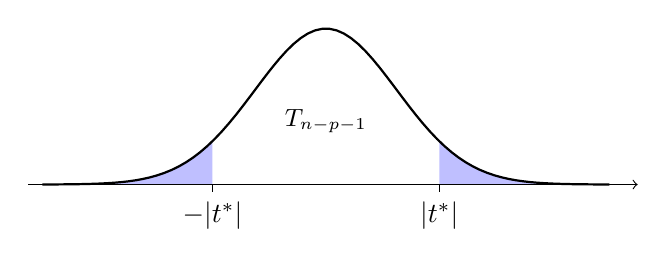
\begin{tikzpicture}[scale=0.9]
    \fill[blue!25,domain=-4:-1.6,samples=40] (-4,0) -- plot (\x,{2.2*exp(-\x*\x/2)}) -- (-1.6,0) -- cycle;
    \fill[blue!25,domain=1.6:4,samples=40] (1.6,0) -- plot (\x,{2.2*exp(-\x*\x/2)}) -- (4,0) -- cycle;
    \draw[->] (-4.2,0) -- (4.4,0);
    \draw[thick,domain=-4:4,samples=80] plot (\x,{2.2*exp(-\x*\x/2)});
    \draw (-1.6,0) -- (-1.6,-0.1) node[below]{$-|t^*|$};
    \draw (1.6,0) -- (1.6,-0.1) node[below]{$|t^*|$};
    \node at (0,0.9) {\small $T_{n-p-1}$};
\end{tikzpicture}
\\[2pt] \textit{\small Two-sided p-value: shaded area in both tails.}
\end{center}

\begin{remark}[CIs and Tests Agree]
    The usual relationship applies: if a 95\% CI does not contain the hypothesized
    value, the null hypothesis would be rejected at the 0.05 significance level.
\end{remark}

\subsection{Example: Room Cleaning Dataset}

\begin{example}[Setup]
    Data from Foster, Stine, and Waterman (1997, p.\ 9): 53 observations. Model the
    number of rooms cleaned ($Y$) by the size of the cleaning crew ($X$).
    \aside{From the scatterplot, constant variance is mildly violated (spread grows with crew size).}
    \\ Step 0: read in data, build the design matrix and response vector (so we can
    also compute manually):
\begin{verbatim}
data <- read.table("cleaning.txt", header=T)
Y <- data[,3]                                 # Rooms Cleaned
X <- as.matrix(cbind(rep(1, 53), data[,2]))   # Predictor: crew size
\end{verbatim}
\end{example}

\begin{example}[Built-in R: \texttt{summary()}]
\begin{verbatim}
model <- lm(Rooms ~ Crews, data=data)
summary(model)

Coefficients:
            Estimate Std. Error t value Pr(>|t|)
(Intercept)   1.7847     2.0965   0.851    0.399
Crews         3.7009     0.2118  17.472   <2e-16 ***
Residual standard error: 7.336 on 51 degrees of freedom
Multiple R-squared: 0.8569, Adjusted R-squared: 0.854
F-statistic: 305.3 on 1 and 51 DF, p-value: < 2.2e-16
\end{verbatim}
    \begin{itemize}
        \item \texttt{Estimate}: $\hat\beta_j$; \texttt{Std.\ Error}: $SE(\hat\beta_j)=\sqrt{\Var(\hat\beta_j)}$
        \item \texttt{t value}: test statistic $t^*=\hat\beta_j/SE(\hat\beta_j)$
        \item \texttt{Pr(>|t|)}: p-value for $H_0:\beta_j=0$ vs.\ $H_A:\beta_j\neq0$
        \item \texttt{Residual standard error}: $s$; degrees of freedom $=n-p-1=53-2=51$
    \end{itemize}
\end{example}

\begin{example}[CIs from the Summary Output]
    CIs are always \rb{estimate} $\pm$ (critical value)$\times$(standard error), with
    estimate $=\hat\beta_j$, critical value $=$ \texttt{qt(alpha/2, df)} or
    \texttt{qt(1-alpha/2, df)}, SE $=SE(\hat\beta_j)$:
\begin{verbatim}
summ  <- summary(model)
coefs <- summ$coefficients   # the 4 columns of summary output
U <- coefs[,1] + qt(0.975, df = 51)*coefs[,2]   # upper bound
L <- coefs[,1] - qt(0.975, df = 51)*coefs[,2]   # lower bound
cbind(L, U)
#                    L        U
# (Intercept) -2.424160 5.993558
# Crews        3.275653 4.126134
\end{verbatim}
\end{example}

\begin{example}[CIs with \texttt{confint()}]
    Defaults to 95\% CIs; works with many model objects (GLMs, nonlinear/weighted least
    squares, \dots); can specify which parameters (default: all).
\begin{verbatim}
confint(model)                  # 95%
confint(model, level=0.9)       # 90%: Crews [3.346039, 4.055748]
confint(model, parm = "Crews")  # only beta1
confint(model, parm = 1)        # by order; 1 is the intercept
\end{verbatim}
\end{example}

\begin{remark}[Term Test Coverage]
    \hlt{\textbf{Term test coverage ends here.}}
\end{remark}

\heading{Study Tips: Transformations and Assumption Checking}
\begin{itemize}
    \item Practice with different datasets.
    \item Generate datasets from distributions that violate the assumptions and check
    residual plots to build intuition.
    \item Try different transformations: which violations get fixed? Which get worse?
    \item Generate datasets that \emph{satisfy} the assumptions and look at their residual
    plots --- what does an acceptable amount of noise/deviation look like?
\end{itemize}

\heading{Rough Guidelines for Transformations}
\begin{itemize}
    \item No universal checklist; it varies from problem to problem.
    \item Issues with \rb{linearity}: consider transforming the \textbf{predictors}.
    \item Issues with \rb{residual variance/distribution}: consider transforming the
    \textbf{response} to stabilize the variance and/or fix the residual distribution.
\end{itemize}

\begin{example}[Room Cleaning: Manual Calculations]
    \textbf{Step 1}: $\hat{\boldsymbol\beta}=(\mathbf{X}'\mathbf{X})^{-1}\mathbf{X}'\mathbf{Y}$
    gives the fitted model $\hat y_i=1.785+3.701x_i$.
\begin{verbatim}
xtx_inv  <- solve(t(X) %*% X)   # (X'X)^-1
xty      <- t(X) %*% Y          # X'Y
beta_hat <- xtx_inv %*% xty     # 1.784699, 3.700893
\end{verbatim}
    \textbf{Step 2}: RSS and $s^2$:
    \[RSS=2744.796,\qquad s^2=\frac{RSS}{n-p-1}=\frac{2744.796}{53-1-1}=53.82\]
\begin{verbatim}
Y_hat <- X %*% beta_hat
RSS   <- sum((Y_hat - Y)^2)     # 2744.796
RSS/51                          # 53.81953
\end{verbatim}
    \textbf{Step 3}: variances. \texttt{xtx\_inv} $=\begin{pmatrix}0.081666 & -0.007235\\ -0.007235 & 0.000834\end{pmatrix}$, so
    \begin{align*}
        \Var(\hat\beta_0)&=s^2(\mathbf{X}'\mathbf{X})^{-1}_{(1,1)}=53.82(0.08167)=4.395\\
        \Var(\hat\beta_1)&=s^2(\mathbf{X}'\mathbf{X})^{-1}_{(2,2)}=53.82(0.00083)=0.0449
    \end{align*}
    \aside{\texttt{s2*xtx\_inv} also gives $\Cov(\hat\beta_0,\hat\beta_1)=-0.3894$.}
    \\ \textbf{Step 4}: critical value and distribution. Sampling distribution is
    $T_{n-p-1}=T_{51}$, $\alpha=0.05$:
    $|t_{0.025,51}|=2.00$ \aside{(\texttt{qt(0.025, 51)} $=-2.007584$)}.
    \\ \textbf{Step 5}: confidence interval:
    \[\hat\beta_0\pm t_{0.025,51}\sqrt{s^2(\mathbf{X}'\mathbf{X})^{-1}_{(1,1)}}=1.785\pm2.00\sqrt{4.395}=[-2.42,\ 5.99]\]
    \textbf{Interpretation}: we are 95\% confident that $\beta_0$ is between $-2.42$ and
    $5.99$. \aside{If we repeat this process with repeated samples, 95\% of the created
    CIs will contain the true $\beta_0$.}
\begin{verbatim}
beta_hat[1] + crit_val*sqrt((s2*xtx_inv)[1,1])   # -2.42416
beta_hat[1] - crit_val*sqrt((s2*xtx_inv)[1,1])   #  5.993558
\end{verbatim}
    \textbf{Step 5 (test)}: in linear regression we almost always test $H_0:\beta_j=0$ vs.\ $H_A:\beta_j\neq0$.
    \[H_0:\beta_1=0:\qquad t^*=\frac{\hat\beta_1-0}{\sqrt{s^2(\mathbf{X}'\mathbf{X})^{-1}_{(2,2)}}}=\frac{3.701}{\sqrt{0.0449}}=17.47\]
    Either compute the p-value or compare with the critical value: $17.47\gg2.00$
    $\Rightarrow$ \dbb{reject $H_0$}; a statistically significant linear relationship exists.
\begin{verbatim}
beta_hat[2]/sqrt((s2*xtx_inv)[2,2])   # 17.47211
2*pt(-17.47, 51)                      # 3.573044e-23
\end{verbatim}
\end{example}

\begin{exercise}[Repeat for $\beta_1$ (CI) and $\beta_0$ (Test)]
    \db{CI for $\beta_1$: $3.701\pm2.0076\sqrt{0.04487}=3.701\pm2.0076(0.2118)=\dbb{[3.276,\ 4.126]}$,
    matching \texttt{confint()}.
    \\ Test for $\beta_0$: $t^*=1.785/\sqrt{4.395}=1.785/2.0965=0.851<2.00$, p-value $=0.399>0.05$
    $\Rightarrow$ \dbb{fail to reject $H_0:\beta_0=0$} (consistent with the CI $[-2.42,5.99]$ containing 0).}
\end{exercise}

\begin{exercise}[Without Matrices]
    Using the data file, repeat the example with the SLR formulas, recalling
    \[\Cov(\hat{\boldsymbol\beta}\mid\mathbf{X})=\frac{\sigma^2}{\sum(x_i-\bar x)^2}\begin{pmatrix}\sum x_i^2/n & -\bar x\\ -\bar x & 1\end{pmatrix},\]
    i.e.\ $\Var(\hat\beta_1)=\dfrac{s^2}{SS_{xx}}$ and $\Var(\hat\beta_0)=s^2\dfrac{\sum x_i^2}{n\,SS_{xx}}=s^2\Big(\dfrac1n+\dfrac{\bar x^2}{SS_{xx}}\Big)$.
\end{exercise}

\subsection{Inference for the Mean Response $E(\mathbf{Y}\mid\mathbf{X})$}

\heading{Three Kinds of Inference with Linear Regression}
\begin{itemize}
    \item On $\boldsymbol\beta$: the relationship between the response and predictors
    \aside{($\boldsymbol\beta$ are unknown population parameters)}.
    \item On $E(\mathbf{Y}\mid\mathbf{X})$, estimated by $\hat{\mathbf{Y}}=\mathbf{X}\hat{\boldsymbol\beta}$
    \aside{(an unknown population parameter, similar to inference on $\mu$ previously)}.
    \item \textbf{Prediction} about an individual observation's $y_0$
    \aside{($y_0$ is an unknown future value)}.
\end{itemize}

\begin{definition}[Estimated Mean Response]
    For each $\mathbf{x}_0'=(1,x_1,x_2,\dots,x_p)$, the estimate is
    \[\hat y_0=\hat E(\mathbf{Y}\mid\mathbf{X}=\mathbf{x}_0')=\mathbf{x}_0'\hat{\boldsymbol\beta}
    =\mathbf{x}_0'(\mathbf{X}'\mathbf{X})^{-1}\mathbf{X}'\mathbf{Y}\]
    This is a \textbf{linear combination of $\mathbf{Y}$}, so we can use
    $\mathbf{Y}\mid\mathbf{X}\sim N_n(\mathbf{X}\boldsymbol\beta,\sigma^2\mathbf{I}_n)$ and
    $\mathbf{A}'\mathbf{Y}\sim N(\mathbf{A}'\boldsymbol\mu,\mathbf{A}'\boldsymbol\Sigma\mathbf{A})$
    with $\mathbf{A}'=\mathbf{x}_0'(\mathbf{X}'\mathbf{X})^{-1}\mathbf{X}'$.
\end{definition}

\begin{proposition}[Sampling Distribution of $\hat y_0$]
    \db{Mean:
    \[E(\hat y_0\mid\mathbf{X},\mathbf{x}_0)=\mathbf{x}_0'(\mathbf{X}'\mathbf{X})^{-1}\mathbf{X}'\,\mathbf{X}\boldsymbol\beta=\mathbf{x}_0'\boldsymbol\beta\]
    Variance, with $\mathbf{A}=\mathbf{X}(\mathbf{X}'\mathbf{X})^{-1}\mathbf{x}_0$:
    \[\Var(\hat y_0\mid\mathbf{X},\mathbf{x}_0)=\mathbf{x}_0'(\mathbf{X}'\mathbf{X})^{-1}\mathbf{X}'\,\sigma^2\mathbf{I}\,\mathbf{X}(\mathbf{X}'\mathbf{X})^{-1}\mathbf{x}_0
    =\sigma^2\mathbf{x}_0'(\mathbf{X}'\mathbf{X})^{-1}\mathbf{x}_0\]
    \aside{Equivalently $\Var(\mathbf{x}_0'\hat{\boldsymbol\beta})=\mathbf{x}_0'\Var(\hat{\boldsymbol\beta})\mathbf{x}_0$.}}
    Hence
    \[\boxed{\hat y_0\mid\mathbf{X},\mathbf{x}_0\sim N\big(\mathbf{x}_0'\boldsymbol\beta,\ \sigma^2\mathbf{x}_0'(\mathbf{X}'\mathbf{X})^{-1}\mathbf{x}_0\big)}\]
    Same issue as before: $\sigma^2$ is unknown, so estimate with $s^2$, which adds
    sampling variability $\Rightarrow$ $T$ distribution:
    \[\boxed{\frac{\hat y_0-\mathbf{x}_0'\boldsymbol\beta}{\sqrt{s^2\mathbf{x}_0'(\mathbf{X}'\mathbf{X})^{-1}\mathbf{x}_0}}\sim T_{n-p-1}}\]
\end{proposition}

\begin{definition}[$(1-\alpha)\%$ CI for the Mean Response $\mathbf{x}_0'\boldsymbol\beta$]
    \[\boxed{\mathbf{x}_0'\hat{\boldsymbol\beta}\pm t_{\alpha/2,\,n-p-1}\;s\sqrt{\mathbf{x}_0'(\mathbf{X}'\mathbf{X})^{-1}\mathbf{x}_0}}\]
    Same $T_{n-p-1}$ distribution as before; a window $2\,t_{\alpha/2,n-p-1}$ standard
    errors wide, centred on the estimate $\mathbf{x}_0'\hat{\boldsymbol\beta}$.
    \\ For SLR the standard error simplifies to
    \[\sqrt{\Var(\hat y_0\mid X,x_0)}=s\sqrt{\frac1n+\frac{(x_0-\bar x)^2}{\sum(x_i-\bar x)^2}}\]
\end{definition}

\begin{exercise}[SLR Standard Error from the Matrix Formula]
    \db{With $\mathbf{x}_0=(1,x_0)'$ and $SS_{xx}=\sum(x_i-\bar x)^2$,
    \begin{align*}
        \mathbf{x}_0'(\mathbf{X}'\mathbf{X})^{-1}\mathbf{x}_0
        &=\frac{1}{SS_{xx}}\Big(\frac{\sum x_i^2}{n}-2x_0\bar x+x_0^2\Big)
        =\frac{1}{SS_{xx}}\Big(\underbrace{\frac{\sum x_i^2}{n}-\bar x^2}_{SS_{xx}/n}+(x_0-\bar x)^2\Big)\\
        &=\frac1n+\frac{(x_0-\bar x)^2}{SS_{xx}}
    \end{align*}
    \aside{The CI is narrowest at $x_0=\bar x$ and widens as $x_0$ moves away from it.}}
\end{exercise}

\begin{definition}[Hypothesis Test for the Mean Response]
    For $H_0:y_0=y_0^0$,
    \[t^*=\frac{\hat y_0-y_0^0}{s\sqrt{\mathbf{x}_0'(\mathbf{X}'\mathbf{X})^{-1}\mathbf{x}_0}}\sim T_{n-p-1}\text{ under }H_0\]
    Think of the mean response as a parameter similar to $\mu$ (the conditional
    population mean for individuals with attributes $\mathbf{x}_0$). Reject $H_0$ if
    $|t^*|>t_{\alpha/2,n-p-1}$, or if $P(|T_{n-p-1}|\geq|t^*|)<\alpha$.
    \aside{Not really done in practice --- usually we create confidence intervals.}
\end{definition}

\begin{example}[Room Cleaning: CI for Mean Response]
    \textit{What is the average number of rooms cleaned with a cleaning crew of size 5?}
    Fitted model $\hat y_i=1.785+3.701x_i$.
\begin{verbatim}
new <- data.frame(Crews=5)   # name must match the original data
predict(model, newdata=new, interval="confidence", level=0.95)
#        fit      lwr      upr
# 1 20.28917 17.73171 22.84662

new <- data.frame(Crews=c(4,2,5))   # several points at once
predict(model, newdata=new, interval="confidence", level=0.95)
#         fit       lwr      upr
# 1 16.588272 13.750660 19.42588
# 2  9.186485  5.699374 12.67360
# 3 20.289166 17.731710 22.84662
\end{verbatim}
\end{example}

\begin{exercise}[Verify the CI Manually]
    Use R to find $(\mathbf{X}'\mathbf{X})^{-1}$, $|t_{0.025,51}|$, $SS_{xx}$, $SS_{yy}$,
    $SP_{xy}$, $\bar X$, $\bar Y$, then complete the calculation with both the SLR and MLR formulas.
    \\\db{MLR: with $\mathbf{x}_0=(1,5)'$,
    $\mathbf{x}_0'(\mathbf{X}'\mathbf{X})^{-1}\mathbf{x}_0=0.081666-2(5)(0.007235)+25(0.000834)=0.03015$, so
    \[SE=\sqrt{53.82(0.03015)}=\sqrt{1.623}=1.274,\qquad 20.289\pm2.0076(1.274)=\dbb{[17.73,\ 22.85]}.\]}
\end{exercise}

\subsection{Prediction Interval for an Actual Response $y_0$}

\begin{remark}[Actual vs.\ Mean Response]
    \begin{itemize}
        \item The regression model gives predicted values \textbf{only} for
        $E(\mathbf{Y}\mid\mathbf{X}=\mathbf{x}_0)$ --- estimates of conditional mean responses.
        We cannot exactly predict any individual response.
        $E(\mathbf{Y}\mid\mathbf{X}=\mathbf{x}_0)$ is a fixed but unknown population parameter.
        \item But an important goal of regression is \textbf{prediction}: for an individual
        with known $\mathbf{x}_0$, what is their $y_0$?
        \item The actual response $y_0$ is a \textbf{realization of a random variable}
        $Y\mid\mathbf{X}=\mathbf{x}_0$: it can take any possible value, and is typically
        not $E(\mathbf{Y}\mid\mathbf{X}=\mathbf{x}_0)$ ($y_0$ is not necessarily on the line/plane
        of best fit). So we must account for the random error as well.
    \end{itemize}
\end{remark}

\begin{definition}[Prediction Error]
    Using $\hat y_0=\mathbf{x}_0'\hat{\boldsymbol\beta}$ as the predicted value,
    \[\boxed{y_0-\hat y_0=\mathbf{x}_0'\boldsymbol\beta+\varepsilon_0-\hat y_0
    =\underbrace{(\mathbf{x}_0'\boldsymbol\beta-\hat y_0)}_{\text{fit of mean}}+\underbrace{\varepsilon_0}_{\text{random error}}}\]
    Two sources of error:
    \begin{itemize}
        \item the random error in the population, $\varepsilon_0$;
        \item how well the model fits the mean response,
        $\mathbf{x}_0'\boldsymbol\beta-\hat y_0=\mathbf{x}_0'\boldsymbol\beta-\mathbf{x}_0'\hat{\boldsymbol\beta}$.
    \end{itemize}
\end{definition}

\begin{proposition}[Distribution of $y_0-\hat y_0$]
    \db{Assuming the model assumptions hold, $\varepsilon_0\sim N(0,\sigma^2)$ for the new
    observation is independent of the sample $\mathbf{Y}$, hence of $\hat y_0$. Mean:
    \[E(y_0-\hat y_0)=\mathbf{x}_0'\boldsymbol\beta+0-\mathbf{x}_0'\boldsymbol\beta=0\]
    Variance (no covariance term, by independence):
    \[\Var(y_0-\hat y_0)=\Var(\varepsilon_0)+\Var(\hat y_0)=\sigma^2+\sigma^2\mathbf{x}_0'(\mathbf{X}'\mathbf{X})^{-1}\mathbf{x}_0\]
    A linear combination of normals is normal, so}
    \[\boxed{y_0-\hat y_0\mid\mathbf{X},\mathbf{x}_0\sim N\big(0,\ \sigma^2[1+\mathbf{x}_0'(\mathbf{X}'\mathbf{X})^{-1}\mathbf{x}_0]\big)}\]
    Estimating $\sigma^2$ with $s^2$ adds sampling variability $\Rightarrow$ $T_{n-p-1}$:
    \[\boxed{\frac{y_0-\hat y_0}{\sqrt{s^2[1+\mathbf{x}_0'(\mathbf{X}'\mathbf{X})^{-1}\mathbf{x}_0]}}\sim T_{n-p-1}}\]
    \hlt{Notice the extra ``$+1$'' term in the variance} (from $\varepsilon_0$).
\end{proposition}

\begin{definition}[$(1-\alpha)\%$ Prediction Interval for $y_0$]
    \[\boxed{\mathbf{x}_0'\hat{\boldsymbol\beta}\pm t_{\alpha/2,\,n-p-1}\;s\sqrt{1+\mathbf{x}_0'(\mathbf{X}'\mathbf{X})^{-1}\mathbf{x}_0}}\]
    \begin{itemize}
        \item We cannot predict the exact value of $y_0$ since we do not know $\epsilon_0$;
        instead give a range of possible values for the actual response.
        \item \textbf{Not} a confidence interval: we are not estimating an unknown
        parameter --- $y_0$ is a realization of a random variable.
        \item Same $T_{n-p-1}$ distribution; window $2\,t_{\alpha/2,n-p-1}$ standard errors
        wide, centred on the estimated mean response $\hat y_0=\mathbf{x}_0'\hat{\boldsymbol\beta}$.
        \item \textbf{Wider} than the CI for the mean response $E(\mathbf{Y}\mid\mathbf{X},\mathbf{x}_0)$.
    \end{itemize}
    For SLR:
    \[\hat\beta_0+\hat\beta_1x_0\pm t_{\alpha/2,\,n-2}\;s\sqrt{1+\frac1n+\frac{(x_0-\bar x)^2}{\sum(x_i-\bar x)^2}}\]
    \aside{Follows from the previous exercise by adding 1 inside the root.}
\end{definition}

\begin{center}
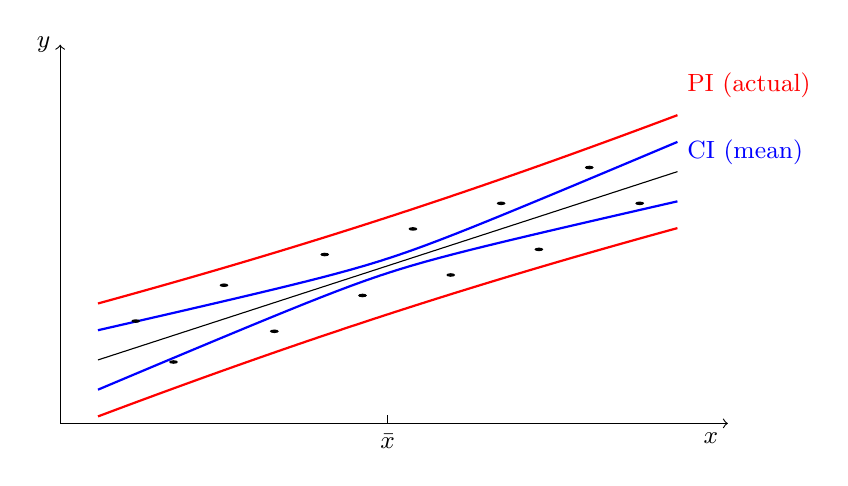
\begin{tikzpicture}[xscale=1.6,yscale=0.65]
    \draw[->] (0,0) -- (5.3,0) node[below left]{\small $x$};
    \draw[->] (0,0) -- (0,7.4) node[left]{\small $y$};
    % PI band (red)
    \draw[red,thick,domain=0.3:4.9,samples=40] plot (\x,{1.0+0.8*\x+sqrt(0.9+0.06*(\x-2.6)^2)});
    \draw[red,thick,domain=0.3:4.9,samples=40] plot (\x,{1.0+0.8*\x-sqrt(0.9+0.06*(\x-2.6)^2)});
    % CI band (blue)
    \draw[blue,thick,domain=0.3:4.9,samples=40] plot (\x,{1.0+0.8*\x+sqrt(0.02+0.06*(\x-2.6)^2)});
    \draw[blue,thick,domain=0.3:4.9,samples=40] plot (\x,{1.0+0.8*\x-sqrt(0.02+0.06*(\x-2.6)^2)});
    \draw[black,domain=0.3:4.9] plot (\x,{1.0+0.8*\x});
    \draw[dashed] (2.6,0) -- (2.6,0.2) node[below=4pt]{\small $\bar x$};
    \foreach \p in {(0.6,1.6+0.4),(0.9,0.8+0.4),(1.3,2.3+0.4),(1.7,1.4+0.4),(2.1,2.9+0.4),(2.4,2.1+0.4),(2.8,3.4+0.4),(3.1,2.5+0.4),(3.5,3.9+0.4),(3.8,3.0+0.4),(4.2,4.6+0.4),(4.6,3.9+0.4)}
        \fill \p circle (1pt);
    \node[blue,right] at (4.9,5.3) {\small CI (mean)};
    \node[red,right] at (4.9,6.6) {\small PI (actual)};
\end{tikzpicture}
\\[2pt] \textit{\small Both bands are centred on the fitted line and narrowest at $\bar x$;
the PI is always wider.}
\end{center}

\begin{example}[Room Cleaning: PI for Actual Response]
    \textit{How many rooms will this cleaning crew of size 5 clean?}
\begin{verbatim}
new <- data.frame(Crews=5)
predict(model, newdata=new, interval="prediction", level=0.95)
#        fit      lwr      upr
# 1 20.28917 5.340774 35.23756

new <- data.frame(Crews=c(4,2,5))
predict(model, newdata=new, interval="prediction", level=0.95)
#         fit       lwr      upr
# 1 16.588272  1.589410 31.58713
# 2  9.186485 -5.948698 24.32167
# 3 20.289166  5.340774 35.23756
\end{verbatim}
    The prediction intervals are \textbf{wider} than the confidence intervals, but the
    \textbf{centres are the same}.
\end{example}

\begin{exercise}[Verify the PI Manually]
    Use R to find $(\mathbf{X}'\mathbf{X})^{-1}$, $|t_{0.025,51}|$, $SS_{xx}$, $SS_{yy}$,
    $SP_{xy}$, $\bar X$, $\bar Y$; do the rest by hand with both the SLR and MLR formulas.
    \\\db{Reusing $\mathbf{x}_0'(\mathbf{X}'\mathbf{X})^{-1}\mathbf{x}_0=0.03015$ at $x_0=5$:
    \[SE=\sqrt{53.82(1+0.03015)}=\sqrt{55.44}=7.446,\qquad 20.289\pm2.0076(7.446)=\dbb{[5.34,\ 35.24]}.\]}
\end{exercise}

\subsection{Confidence vs.\ Prediction Intervals}

\begin{center}
    \begin{tabular}{p{0.44\linewidth}p{0.44\linewidth}}
        \toprule
        \textbf{Confidence interval} & \textbf{Prediction interval} \\
        \midrule
        For the \textbf{mean response} & For a \textbf{future/specific observation} \\[2pt]
        ``What would be the average selling price for a house with characteristics $\mathbf{x}_0$?''
        & ``What is the predicted sale price for \emph{this} house with characteristics $\mathbf{x}_0$?'' \\[2pt]
        SE: $s\sqrt{\mathbf{x}_0'(\mathbf{X}'\mathbf{X})^{-1}\mathbf{x}_0}$
        & SE: $s\sqrt{1+\mathbf{x}_0'(\mathbf{X}'\mathbf{X})^{-1}\mathbf{x}_0}$ \\
        \bottomrule
    \end{tabular}
\end{center}
\begin{itemize}
    \item Prediction intervals are \textbf{always wider} than confidence intervals
    \aside{(think: variability of $y_i$ vs.\ $\bar y$)} --- they include variation in
    estimating the conditional mean \emph{and} variation around the conditional mean.
    \item Both are centred at $\mathbf{x}_0'\hat{\boldsymbol\beta}$.
    \item Some sources call both ``confidence intervals'' but specify whether the
    interest is a single future response or the mean response.
\end{itemize}

\begin{remark}[Module Takeaways]
    \begin{itemize}
        \item How did we determine the properties of the sampling distribution, and where
        did the assumptions play a role?
        \item Why do we use a $T$ distribution with the sampling distribution in practice?
        \item How do we compute confidence/prediction intervals and conduct hypothesis
        tests on regression components?
        \item How are the inferential procedures concluded?
        \item What is the difference between estimating a mean response and predicting an
        actual response?
    \end{itemize}
    \aside{Next week: variance decomposition --- how much of the total variation is
    explained by the predictors?}
\end{remark}
